% Template for PLoS
% Version 3.1 February 2015
%
% % % % % % % % % % % % % % % % % % % % % % %
%
% -- FIGURES AND TABLES
%
% DO NOT INCLUDE GRAPHICS IN YOUR MANUSCRIPT
% - Figures should be uploaded separately from your manuscript file. 
% - Figures generated using LaTeX should be extracted and removed from the PDF before submission. 
% - Figures containing multiple panels/subfigures must be combined into one image file before submission.
% For figure citations, please use "Fig." instead of "Figure".
% See http://www.plosone.org/static/figureGuidelines for PLOS figure guidelines.
%
% Tables should be cell-based and may not contain:
% - tabs/spacing/line breaks within cells to alter layout or alignment
% - vertically-merged cells (no tabular environments within tabular environments, do not use \multirow)
% - colors, shading, or graphic objects
% See http://www.plosone.org/static/figureGuidelines#tables for table guidelines.
%
% % % % % % % % % % % % % % % % % % % % % % % 

\documentclass[10pt,letterpaper]{article}\usepackage[]{graphicx}\usepackage[]{color}
%% maxwidth is the original width if it is less than linewidth
%% otherwise use linewidth (to make sure the graphics do not exceed the margin)
\makeatletter
\def\maxwidth{ %
  \ifdim\Gin@nat@width>\linewidth
    \linewidth
  \else
    \Gin@nat@width
  \fi
}
\makeatother

\definecolor{fgcolor}{rgb}{0.345, 0.345, 0.345}
\newcommand{\hlnum}[1]{\textcolor[rgb]{0.686,0.059,0.569}{#1}}%
\newcommand{\hlstr}[1]{\textcolor[rgb]{0.192,0.494,0.8}{#1}}%
\newcommand{\hlcom}[1]{\textcolor[rgb]{0.678,0.584,0.686}{\textit{#1}}}%
\newcommand{\hlopt}[1]{\textcolor[rgb]{0,0,0}{#1}}%
\newcommand{\hlstd}[1]{\textcolor[rgb]{0.345,0.345,0.345}{#1}}%
\newcommand{\hlkwa}[1]{\textcolor[rgb]{0.161,0.373,0.58}{\textbf{#1}}}%
\newcommand{\hlkwb}[1]{\textcolor[rgb]{0.69,0.353,0.396}{#1}}%
\newcommand{\hlkwc}[1]{\textcolor[rgb]{0.333,0.667,0.333}{#1}}%
\newcommand{\hlkwd}[1]{\textcolor[rgb]{0.737,0.353,0.396}{\textbf{#1}}}%

\usepackage{framed}
\makeatletter
\newenvironment{kframe}{%
 \def\at@end@of@kframe{}%
 \ifinner\ifhmode%
  \def\at@end@of@kframe{\end{minipage}}%
  \begin{minipage}{\columnwidth}%
 \fi\fi%
 \def\FrameCommand##1{\hskip\@totalleftmargin \hskip-\fboxsep
 \colorbox{shadecolor}{##1}\hskip-\fboxsep
     % There is no \\@totalrightmargin, so:
     \hskip-\linewidth \hskip-\@totalleftmargin \hskip\columnwidth}%
 \MakeFramed {\advance\hsize-\width
   \@totalleftmargin\z@ \linewidth\hsize
   \@setminipage}}%
 {\par\unskip\endMakeFramed%
 \at@end@of@kframe}
\makeatother

\definecolor{shadecolor}{rgb}{.97, .97, .97}
\definecolor{messagecolor}{rgb}{0, 0, 0}
\definecolor{warningcolor}{rgb}{1, 0, 1}
\definecolor{errorcolor}{rgb}{1, 0, 0}
\newenvironment{knitrout}{}{} % an empty environment to be redefined in TeX

\usepackage{alltt}
\usepackage[top=0.85in,left=2.75in,footskip=0.75in]{geometry}

% Use adjustwidth environment to exceed column width (see example table in text)
\usepackage{changepage}

% Use Unicode characters when possible
\usepackage[utf8]{inputenc}

% textcomp package and marvosym package for additional characters
\usepackage{textcomp,marvosym}

% fixltx2e package for \textsubscript
\usepackage{fixltx2e}

% amsmath and amssymb packages, useful for mathematical formulas and symbols
\usepackage{amsmath,amssymb}

% cite package, to clean up citations in the main text. Do not remove.
\usepackage{cite}

% Use nameref to cite supporting information files (see Supporting Information section for more info)
\usepackage{nameref}

% line numbers
\usepackage[right]{lineno}

% ligatures disabled
\usepackage{microtype}
\DisableLigatures[f]{encoding = *, family = * }

% rotating package for sideways tables
\usepackage{rotating}

% packages I added
\usepackage{cleveref}
\usepackage[colorlinks=true,allcolors=Gray]{hyperref}
\usepackage[usenames,dvipsnames]{xcolor}

% Remove comment for double spacing
%\usepackage{setspace} 
%\doublespacing

% Text layout
\raggedright
\setlength{\parindent}{0.5cm}
\textwidth 5.25in 
\textheight 8.75in

% Bold the 'Figure #' in the caption and separate it from the title/caption with a period
% Captions will be left justified
\usepackage[aboveskip=1pt,labelfont=bf,labelsep=period,justification=raggedright,singlelinecheck=off]{caption}

% Use the PLoS provided BiBTeX style
\bibliographystyle{plos2015}

% Remove brackets from numbering in List of References
\makeatletter
\renewcommand{\@biblabel}[1]{\quad#1.}
\makeatother

% Leave date blank
\date{}

% Header and Footer with logo
\usepackage{lastpage,fancyhdr,graphicx}
\usepackage{epstopdf}
\pagestyle{myheadings}
\pagestyle{fancy}
\fancyhf{}
\lhead{\includegraphics[width=2.0in]{PLOS-submission.eps}}
\rfoot{\thepage/\pageref{LastPage}}
\renewcommand{\footrule}{\hrule height 2pt \vspace{2mm}}
\fancyheadoffset[L]{2.25in}
\fancyfootoffset[L]{2.25in}
\lfoot{\sf PLOS}

% for acronyms
\usepackage{acronym}

%% Include all macros below

% cleveref options
\crefname{table}{Table}{Tables}
\crefname{figure}{Fig.}{Figs.}
\renewcommand{\figurename}{Fig.}

% acronyms
\acrodef{CDMO}{Centralized Data Management Office}
\acrodef{CRAN}{Comprehensive R Archive Network}
\acrodef{DO}{dissolved oxygen}
\acrodef{NERRS}{National Estuarine Research Reserve System}
\acrodef{QAQC}{quality assurance/quality control}
\acrodef{SWMP}{System Wide Monitoring Program}

%% END MACROS SECTION

%knitr options


\IfFileExists{upquote.sty}{\usepackage{upquote}}{}
\begin{document}
\vspace*{0.35in}
\urlstyle{same}

% Title must be 250 characters or less.
% Please capitalize all terms in the title except conjunctions, prepositions, and articles.
\begin{flushleft}
{\Large
\textbf\newline{SWMPr: An R Package for Retrieving, Organizing, and Analyzing Environmental Data for Estuaries}
}
\newline
% Insert author names, affiliations and corresponding author email (do not include titles, positions, or degrees).
\\
Marcus William Beck\textsuperscript{1, *}

\bigskip
\bf{1} ORISE Research Participation Program, USEPA National Health and Environmental Effects Research Laboratory, Gulf Ecology Division, 1 Sabine Island Drive, Gulf Breeze, FL 32651, USA
\\
\bigskip

* beck.marcus@epa.gov

\end{flushleft}

\section*{Abstract}
Standardized monitoring programs have vastly improved the quantity and quality of data that form the basis of environmental decision-making.  One example in the United States is the \ac{SWMP} that was implemented in 1995 by the federally-funded \ac{NERRS}.  This program has provided two decades of continuous monitoring data at over 140 fixed stations in 28 estuaries.  \ac{SWMP} data have been used in a variety of applications with the general objective of describing dynamics of estuarine ecosystems to better inform effective coastal management.  However, simple tools for processing and evaluating the increasing quantity of data provided by the monitoring network have prevented broad-scale comparisons between systems and, in some cases, simple trend analysis of water quality parameters at individual sites.  I describe SWMPr, an open-source R package, for use with \ac{SWMP} environmental data.  The package provides several functions that facilitate data retrieval, organization, and analysis of time series data to describe water quality, weather, and nutrient dynamics in the reserve estuaries.  Previously unavailable functions for estuaries are also provided to estimate rates of ecosystem metabolism using the open-water method.  Tools included with the SWMPr package have facilitated a cross-reserve comparison of trends, including simple evaluation of changes over time and comparisons of patterns in primary productivity.  Overall, the package provides an effective approach to link quantitative information with analysis tools that will greatly inform management programs aimed at coastal protection and restoration.

\linenumbers

\section*{Introduction}

The development of low-cost, automated sensors that collect data in near real-time has enabled a proliferation of standardized environmental monitoring programs \cite{Glasgow04,Fries08}.  These programs provide access to invaluable sources of data that can be used to address a variety of research and management objectives.  Applications from automated remote sensors are numerous for aquatic environments with notable examples including prediction of harmful algal blooms and toxicants in freshwater systems \cite{Reed10}, development of a hydrometeorological monitoring network to support flash flood warning programs \cite{HADS15}, and a national marine buoy network covering large portions of the open ocean and coastal zones of the United States \cite{NDBC15}.  Automated remote monitoring programs offer several advantages over traditional site-specific, field-based methods including streamlining of data acquisition, minimizing human error, and reducing the overall cost of the collection process \cite{Glasgow04}.  However, the increasing quantity of available information to address relevant questions has contributed to the growth of `big data' where analyses are limited by compututational requirements and identifying the signal from the noise rather than the availability of information. A greater focus on synthesis, exploratory-based analytical techniques, and interpretation have characterized the use of data from automated monitoring programs \cite{Campbell13,Millie13}.

An important monitoring network for coastal environments in the United States is the \acl{NERRS} (\acs{NERRS})\footnote{\url{http://www.nerrs.noaa.gov/}}.  This network represents 28 estuarine reserves from different biogeographic regions that were chosen to address multiple goals for long-term research, monitoring, education, and stewardship in support of coastal management.  As part of this effort, the \acf{SWMP}\footnote{\url{http://nerrs.noaa.gov/RCDefault.aspx?ID=18}} was implemented in 1995 at over 140 stations at the reserves to provide a robust, long-term monitoring system for water quality, weather, and land-use/habitat change.  The \ac{SWMP} network has provided a continuous source of data collected at near real-time with the intent to evaluate natural and anthropogenic causes of spatiotemporal variation in environmental condition and ecosystem function.  These data have been applied both for evaluations of relevant characteristics at individual reserves (eg., \cite{Bulthius95,Dix08}) and differences between reserves (e.g., ecosystem metabolism \cite{Caffrey03,Caffrey04}, tidal characteristics \cite{Sanger02}, dissolved oxygen \cite{Wenner04}).  However, no cross-reserve comparisons have been conducted within the last decade despite the online availability of current \ac{SWMP} data.  \ac{NERRS} researchers and staff have also expressed a need for quantitative analysis tools to evaluate trends in water quality time series given the quantity and quality of data provided by \ac{SWMP} \cite{SWMP14}.          

This article describes a software package that was developed to address research needs of the \ac{NERRS} program using the open-source statistical programming language R \cite{RDCT14}.  SWMPr (pronounced `swamper') is an R package that contains functions for retrieving, organizing, and analyzing estuary monitoring data from the \acl{SWMP}.  Functions provided by SWMPr address many of the common issues working with large datasets created from automated sensor networks, such as data pre-processing to remove unwanted information, combining data from different sources, and exploratory analyses to identify key parameters of interest.  Additionally, a cross-reserve comparison of water quality trends and current ecosystem metabolism estimates is provided to illustrate potential applications using the functions in this package.  The software is provided specifically for use with \ac{NERRS} data, although many of the applications are relevant for addressing common challenges working with large datasets.

\section*{SWMP overview and data retrieval}

Four core data elements are collected through the \ac{SWMP} monitoring network: abiotic monitoring data, biotic observations, habitat and land use mapping, and sentinel monitoring.  Only the abiotic data are monitored continuously with automated sensor networks, whereas the remaining elements involve field surveys or mapping products that differ between reserves given site-specific requirements.  As such, the SWMPr package is developed for the continuous abiotic monitoring network that represents a majority of the \ac{SWMP} data and, consequently, the most challenging to evaluate.  Abiotic elements monitored at each reserve include water quality (water temperature, specific conductivity, salinity, dissolved oxygen concentration, dissolved oxygen saturation, depth, pH, turbidity, chlorophyll fluorescence), weather (air temperature, relative humidity, barometric pressure, wind speed, wind direction, photosynthetically active radiation, precipitation), and nutrient data (orthophosphate, ammonium, nitrite, nitrate, nitrite + nitrate, chlorophyll a).  Each reserve has no less than four water quality stations and one weather station at fixed locations.  Water quality and weather data are collected at 15 minute intervals, whereas nutrient data are collected monthly at each water quality station.  All data are made accessible through the \ac{CDMO} web portal\footnote{\url{http://cdmo.baruch.sc.edu/}}, where multiple \ac{QAQC} measures are used to screen the information for accuracy and reliability.  The final data include all timestamped observations including relevant \ac{QAQC} flags with the appropriate qualifier.

The \ac{CDMO} web portal was established to support priority areas of \ac{SWMP} that focus on the continuation and advancement of data management.  As such, \ac{CDMO} provides access to over 35 million water quality, weather, and nutrient records that have been authenticated through systematic \ac{QAQC} procedures.    Prior to any data request to the \ac{CDMO}, the location, parameter type, and date ranges need to be identified based on the analysis needs. All stations in the \ac{SWMP} network are identified by a 7 or 8 character name that specifies the reserve, station, and parameter type.  For example, `apaebwq' is the water quality identifier (`wq') for the East Bay station (`eb') at the Apalachicola reserve (`apa').  Similarly, a suffix of `met' or `nut' would specify the weather (meteorological) or nutrients station.  All reserve names, stations, and date ranges for each parameter type can be viewed on the \ac{CDMO} website. Alternatively, the \texttt{site\_codes} (all sites) or \texttt{site\_codes\_ind} (single site) functions provided by the SWMPr package can be used to view the same information.  As noted below, the computer's IP address must be registered with \ac{CDMO} before using the data retrieval functions in SWMPr.  Web services\footnote{\url{http://cdmo.baruch.sc.edu/webservices.cfm}} are provided by \ac{CDMO} for direct access to \ac{SWMP} data through http requests, in addition to standard graphical user interface options for selecting data.  The data retrieval functions in SWMPr are simple calls to the existing retrieval functions on \ac{CDMO} web services.  For example, the \texttt{site\_codes} function in SWMPr uses the \texttt{exportStationCodesXMLNew} function from the web services to retrieve metadata for all the \ac{SWMP} sites.  The text below describes the data retrieval functions in more detail, including all other functions available in SWMPr.

\section*{Structure of the SWMPr package}

\subsection*{Installing the package}

The SWMPr package was developed for use with the R ($\geq$ v3.0.0) statistical programming language \cite{RDCT14}. The SWMPr package can be downloaded from the \ac{CRAN}\footnote{\url{http://cran.r-project.org/web/packages/SWMPr/index.html} for the \ac{CRAN} release, the development version can be installed  from \url{https://github.com/fawda123/SWMPr}.} by executing the following commands at the R console prompt.  The package is loaded in the workspace using the \texttt{library} command.

\begin{knitrout}\small
\definecolor{shadecolor}{rgb}{1, 1, 1}\color{fgcolor}\begin{kframe}
\begin{verbatim}
> install.packages('SWMPr')
> library(SWMPr)
\end{verbatim}
\end{kframe}
\end{knitrout}


The SWMPr package was developed by considering a standard workflow that categorizes the functions as one of three steps based on their intended use: retrieving, organizing, and analyzing.  Functions for retrieving are used to import the data into R as a \texttt{swmpr} object class.  Functions for organizing and analyzing the data provide methods for working with a \texttt{swmpr} object.  An additional group of `miscellaneous' functions are included as helpers for the main functions.  The following describes the package structure, beginning with the retrieval functions, a description of the \texttt{swmpr} object returned after retrieval, and, finally, the organizing and analyzing functions.

\subsection*{Data retrieval}

Two approaches can be used to import \ac{SWMP} data into R, either through direct download or by importing local data (\Cref{tab:retrieve}). First, functions from the package can be used to import the data directly from the online server using \ac{CDMO} web services. To do so, the IP address for the computer making the request must be registered with \ac{CDMO}.\footnote{Follow instructions here: \url{http://cdmo.baruch.sc.edu/webservices.cfm}}  The \texttt{site\_codes} or \texttt{site\_codes\_ind} functions can be used to view the available metadata after a computer is registered with \ac{CDMO}. 

% table for retrieval functions
%latex.default(to_tab[, "Description", drop = F], file = "", caption = "Retrieval functions available from the SWMPr package. Full documentation for each function is in the help file (e.g., execute \\texttt{?all\\_params} for individual functions or \\texttt{help.search(`retrieve', package = `SWMPr')} for all).",     rowlabel = "Function", colheads = "Description", rowname = to_tab$Functions,     caption.loc = "top", col.just = c("p{3.5in}"), label = "tab:retrieve",     table.env = FALSE)%
\begin{table}[!tbp]
\caption{Retrieval functions available from the SWMPr package. Full documentation for each function is in the help file (e.g., execute \texttt{?all\_params} for individual functions or \texttt{help.search(`retrieve', package = `SWMPr')} for all).\label{tab:retrieve}} 
\begin{center}
\begin{tabular}{lp{3.5in}}
\hline\hline
\multicolumn{1}{l}{Function}&\multicolumn{1}{c}{Description}\tabularnewline
\hline
\texttt{all\_params}&Retrieve records starting with the most recent at a given station, all parameters.  Wrapper to \texttt{exportAllParamsXMLNew} function on web services.\tabularnewline
\texttt{all\_params\_dtrng}&Retrieve records of all parameters within a given date range for a station.  Optional argument for a single parameter. Wrapper to \texttt{exportAllParamsDateRangeXMLNew}.\tabularnewline
\texttt{import\_local}&Import files from a local path.  The files must be in a specific format, such as those returned from the \ac{CDMO} using the zip downloads option.\tabularnewline
\texttt{single\_param}&Retrieve records for a single parameter starting with the most recent at a given station.  Wrapper to \texttt{exportSingleParamXMLNew} function on web services.\tabularnewline
\texttt{site\_codes}&Metadata for all stations, wrapper to \texttt{exportStationCodesXMLNew} function on web services.\tabularnewline
\texttt{site\_codes\_ind}&Metadata for all stations at a single site, wrapper  to \texttt{NERRFilterStationCodesXMLNew} function on web services.\tabularnewline
\hline
\end{tabular}\end{center}

\end{table}


\begin{knitrout}\small
\definecolor{shadecolor}{rgb}{1, 1, 1}\color{fgcolor}\begin{kframe}
\begin{verbatim}
> # retrieve metadata for all sites
> site_codes()
> 
> # retrieve metadata for a single site
> site_codes_ind('apa')
\end{verbatim}
\end{kframe}
\end{knitrout}

Data retrieval functions to import data directly into R from the \ac{CDMO} include \texttt{all\_params}, \texttt{all\_params\_dtrng}, and \texttt{single\_param}: \texttt{all\_params} returns the most recent records of all parameters at a station, \texttt{all\_params\_dtrng} returns all records within a date range for all parameters or a single parameter, and \texttt{single\_param} is identical to \texttt{all\_params} except that a single parameter is requested. Due to rate limitations on the \ac{CDMO} server, the retrieval functions return a limited number of records with each request.  However, the SWMPr functions use the native CDMO web services iteratively (i.e., within a loop) to obtain the desired time series.  Download time can be excessive for longer time series.     

\begin{knitrout}\small
\definecolor{shadecolor}{rgb}{1, 1, 1}\color{fgcolor}\begin{kframe}
\begin{verbatim}
> # all parameters for a station, most recent
> all_params('hudscwq')
> 
> # get all parameters within a date range
> all_params_dtrng('hudscwq', c('09/10/2012', '02/8/2013'))
> 
> # get single parameter within a date range
> all_params_dtrng('hudscwq', c('09/10/2012', '02/8/2013'), 
+   param = 'do_mgl')
> 
> # single parameter for a station, most recent
> single_param('hudscwq', 'do_mgl')
\end{verbatim}
\end{kframe}
\end{knitrout}

The second approach for data retrieval is to use the \texttt{import\_local} function to import data into R that are locally available after downloading from \ac{CDMO}.  This approach is most appropriate for large, specific data requests. The \texttt{import\_local} function is designed for data from the zip downloads\footnote{\url{http://cdmo.baruch.sc.edu/aqs/zips.cfm}} feature in the advanced query section of the \ac{CDMO}. The zip downloads feature can be used to obtain data from multiple stations in one request.  The downloaded data will be in a compressed folder that includes multiple .csv files by year for a given data type (e.g., apacpwq2002.csv, apacpwq2003.csv, apacpnut2002.csv, etc.).  The \texttt{import\_local} function can be used to import files directly from the zipped folder or after the folder is decompressed

Occasionally, non-unique observations are present in the raw data.  These duplicates may be actual replicates with unique time stamps, such as replicate samples for monthly nutrient data.  Erroneous duplicates with non-unique time stamps may also be present.  The \texttt{import\_local} function handles duplicate entries differently depending on the data type.  For water quality and nutrient data, duplicate time stamps are simply removed.  Nutrient data often contain replicate samples with similar but not identical time stamps within the span of a few minutes.  Nutrient data with replicates with unique time stamps are not removed but can be further processed using \texttt{rem\_reps}.  Weather data prior to 2007 may also contain duplicate time stamps at frequencies for hourly (denoted as `60') and daily (`144') averages, in addition to 15 minute frequencies.  Only duplicate values at 15 minutes are averaged for weather data during import.  

\begin{knitrout}\small
\definecolor{shadecolor}{rgb}{1, 1, 1}\color{fgcolor}\begin{kframe}
\begin{verbatim}
> # import local data for apaebmet
> 
> # this is an example path with the decompressed csv files
> path <- 'C:/my_path/'
> 
> # import, do not include file extension
> import_local(path, 'apadbwq') 
\end{verbatim}
\end{kframe}
\end{knitrout}

\subsection*{The \texttt{swmpr} object class}

All data retrieval functions return a \texttt{swmpr} object that includes relevant data and several attributes describing the dataset.  The data include a \texttt{datetimestamp} column in the appropriate timezone for a station and additional parameters for a given data type (weather, nutrients, or water quality).  Correspondingg \ac{QAQC} columns for each parameter are also returned if provided by the initial data request.  The following shows an example of the raw data imported using \texttt{all\_params}.

\begin{knitrout}\small
\definecolor{shadecolor}{rgb}{1, 1, 1}\color{fgcolor}\begin{kframe}
\begin{verbatim}
> # import all paramaters for the station
> # three most recent records
> exdat <- all_params('apadbwq', Max = 3, trace = F)
> exdat
##         datetimestamp temp f_temp spcond f_spcond sal f_sal do_pct
## 1 2015-04-21 13:00:00   21      0   0.07        0   0     0     99
## 2 2015-04-21 13:15:00   21      0   0.05        0   0     0     99
## 3 2015-04-21 13:30:00   22      0   0.03        0   0     0     98
##   f_do_pct do_mgl f_do_mgl depth f_depth ph f_ph turb f_turb chlfluor
## 1        0      9        0  0.02       0  8    0    2      0       NA
## 2        0      9        0  0.02       0  8    0    2      0       NA
## 3        0      8        0  0.02       0  8    0   16      0       NA
##   f_chlfluor level f_level cdepth clevel f_cdepth f_clevel
## 1         -2    NA      -1  -0.01     NA        3         
## 2         -2    NA      -1   0.00     NA        3         
## 3         -2    NA      -1   0.00     NA        3
\end{verbatim}
\end{kframe}
\end{knitrout}

The attributes for a \texttt{swmpr} object are descriptors that are appended to the raw data (\cref{tab:attributes}).  These act as metadata that are used internally by many of the package functions and are updated as the data are processed. The attributes are not visible with the raw data but can be viewed as follows.

\begin{knitrout}\small
\definecolor{shadecolor}{rgb}{1, 1, 1}\color{fgcolor}\begin{kframe}
\begin{verbatim}
> # import sample data from package
> data(apadbwq)
> dat <- apadbwq
> 
> # view all attributes of dat
> attributes(dat)
>  
> # view a single attribute of dat
> attr(dat, 'station')
\end{verbatim}
\end{kframe}
\end{knitrout}
 
% attributes table
%latex.default(to_tab[, -1, drop = F], file = "", caption = "Attributes of a \\texttt{swmpr} object that describe characteristics of the data.",     rowlabel = "Attributes", colheads = c("Class", "Description"),     rowname = to_tab$Attributes, caption.loc = "top", insert.bottom = foot,     col.just = c("p{0.75in}", "p{3.25in}"), label = "tab:attributes",     table.env = FALSE)%
\begin{table}[!tbp]
\caption{Attributes of a \texttt{swmpr} object that describe characteristics of the data.\label{tab:attributes}} 
\begin{center}
\begin{tabular}{lp{0.75in}p{3.25in}}
\hline\hline
\multicolumn{1}{l}{Attributes}&\multicolumn{1}{c}{Class}&\multicolumn{1}{c}{Description}\tabularnewline
\hline
\texttt{names}&character&Column names of the entire data set, inherited from the \texttt{data.frame} object class\tabularnewline
\texttt{row.names}&integer&Row names of the data set, inherited from the \texttt{data.frame} object class\tabularnewline
\texttt{class}&character&Class of the data object indicating \texttt{swmpr} and \texttt{data.frame}\tabularnewline
\texttt{station}&character&Station identifier used by \ac{NERRS} as a string with 7 or 8 characters\tabularnewline
\texttt{parameters}&character&Character vector of column names for data parameters, e.g., \texttt{`do\_mgl'}\tabularnewline
\texttt{qaqc\_cols}&logical&Indicates if \ac{QAQC} columns are present in the raw data\tabularnewline
\texttt{date\_rng}&POSIXct&Start and end dates for the raw data\tabularnewline
\texttt{timezone}&character&Timezone of the station using the city/country format\textsuperscript{\textit{a}}\tabularnewline
\texttt{stamp\_class}&character&Class of the \texttt{datetimestamp} column, usually POSIXct unless data have been aggregated\tabularnewline
\hline
\end{tabular}\end{center}

\textsuperscript{\textit{a}}\footnotesize Time zones that do not observe daylight savings are used for \texttt{swmpr} objects and may not be cities in the United States.  For example, ``America/Jamaica" is used for Eastern Standard Time.\end{table}


The \texttt{swmpr} object class was created for use with the organizing and analyzing functions.  This object-oriented approach is standard for R (i.e., the S3 object  system, \cite{Wickham14}), such that specific methods for a generic function are developed for the object class.  A \texttt{swmpr} object also secondarily inherits methods from the \texttt{data.frame} class, such that common \texttt{data.frame} methods also apply to \texttt{swmpr} objects.  Available methods for the \texttt{swmpr} class are described below and can also be viewed:
 
\begin{knitrout}\small
\definecolor{shadecolor}{rgb}{1, 1, 1}\color{fgcolor}\begin{kframe}
\begin{verbatim}
> # view available methods for swmpr class
> methods(class = 'swmpr')
\end{verbatim}
\end{kframe}
\end{knitrout}

A sample dataset can be downloaded for use with the examples below.\footnote{\url{https://s3.amazonaws.com/swmpexdata/zip_ex.zip}}  This dataset has an identical format as the data returned from the zip downloads feature of the \ac{CDMO}.  Processed verions of the raw data are also included with the package as binary data files (RData).  These include \texttt{swmpr} objects for four stations at Apalachicola Bay: apacpnut, apacpwq, apadbwq, and apaebmet.  Information for each file can be viewed in the help documentation (e.g., \texttt{?apacpnut}).

\subsection*{Data organizing}

The organize functions are used to clean or prepare the imported data for analysis, including viewing and removal of QAQC flags, subsetting, combining replicate nutrient observations, creating a standardized time series, and combining data of different types (\Cref{tab:organize}).

The \texttt{qaqc} function is a simple screen to retain observations from the data with specified QAQC flags.\footnote{\ac{CDMO} flags: \url{http://cdmo.baruch.sc.edu/data/qaqc.cfm}} Each parameter in the imported \texttt{swmpr} object will have a corresponding QAQC column of the same name with the added prefix \texttt{f\_} (e.g., \texttt{do\_mgl}, \texttt{f\_do\_mgl}).  Values in the QAQC column range from -5 to 5 to indicate the \ac{QAQC} flag that was assigned by \ac{CDMO} during initial processing.  The \ac{QAQC} function is used to remove observations in the raw data with given flags, with the default option to retain only values with the \texttt{0} \ac{QAQC} flag (i.e., passed initial \ac{CDMO} checks).     Additionally, simple filters are used to remove obviously bad values, e.g., wind speed values less than zero or pH values greater than 12. Erroneous data entered as -99 are also removed. The function returns the original data with the QAQC columns removed and \texttt{NA} (not available) values for observations that do not meet the criteria specified in the function call.

% table for organize functions
%latex.default(to_tab[, "Description", drop = F], file = "", caption = "Organizing functions available from the SWMPr package. Full documentation for each function is in the help file (e.g., execute \\texttt{?comb} for individual functions or \\texttt{help.search(`organize', package = `SWMPr')} for all).",     rowlabel = "Function", colheads = "Description", rowname = to_tab$Functions,     caption.loc = "top", col.just = c("p{3.5in}"), label = "tab:organize",     table.env = FALSE)%
\begin{table}[!tbp]
\caption{Organizing functions available from the SWMPr package. Full documentation for each function is in the help file (e.g., execute \texttt{?comb} for individual functions or \texttt{help.search(`organize', package = `SWMPr')} for all).\label{tab:organize}} 
\begin{center}
\begin{tabular}{lp{3.5in}}
\hline\hline
\multicolumn{1}{l}{Function}&\multicolumn{1}{c}{Description}\tabularnewline
\hline
\texttt{comb}&Combines \texttt{swmpr} objects to a common time series using setstep, such as combining the weather, nutrients, and water quality data for a single station. Only different data types can be combined.\tabularnewline
\texttt{qaqc}&Remove \ac{QAQC} columns and remove data based on \ac{QAQC} flag values for a \texttt{swmpr} object.  Only applies if \ac{QAQC} columns are present. \tabularnewline
\texttt{qaqcchk}&View a summary of the number of observations in a \texttt{swmpr} object that are assigned to different \ac{QAQC} flags used by \ac{CDMO}.  The output can be used to inform further processing.\tabularnewline
\texttt{rem\_reps}&Remove replicate nutrient data that occur on the same day.  The default is to average replicates.\tabularnewline
\texttt{setstep}&Format data from a \texttt{swmpr} object to a continuous time series at a given timestep.  The function is used in \texttt{comb} and can also be used with individual stations.\tabularnewline
\texttt{subset}&Subset by dates and/or columns for a \texttt{swmpr} object.  This is a method passed to the generic \texttt{subset} function provided in the base package.\tabularnewline
\hline
\end{tabular}\end{center}

\end{table}


\begin{knitrout}\small
\definecolor{shadecolor}{rgb}{1, 1, 1}\color{fgcolor}\begin{kframe}
\begin{verbatim}
> # qaqc screen for a swmpr object, retain only '0'
> qaqc(dat)
> 
> # retain all data regardless of flag
> qaqc(dat, qaqc_keep = NULL)
> 
> # retain only '0' and '-1' flags
> qaqc(dat, qaqc_keep = c(0, -1))
\end{verbatim}
\end{kframe}
\end{knitrout}

Viewing the number of observations for each parameter that are assigned to a \ac{QAQC} flag may be useful for deciding how to process the data with \texttt{qaqc}.  The \texttt{qaqcchk} function can be used to view this information.

\begin{knitrout}\small
\definecolor{shadecolor}{rgb}{1, 1, 1}\color{fgcolor}\begin{kframe}
\begin{verbatim}
> # view the number of observations in each QAQC flag
> qaqcchk(dat)
\end{verbatim}
\end{kframe}
\end{knitrout}

Raw nutrient data obtained from the \ac{CDMO} will usually include replicate samples that were taken within a few minutes of each other.  The \texttt{rem\_reps} function combines nutrient data that occur on the same day to preserve an approximate monthly time step.  The \texttt{datetimestamp} column will always be averaged for replicates, but the actual observations will be combined based on the user-supplied function which defaults to the mean.  Other suggested functions include the \texttt{median}, \texttt{min}, or \texttt{max}.  The entire function call, including treatment of \texttt{NA}, values should be passed to the \texttt{FUN} argument (see the examples).  The function is meant to be used after \texttt{qaqc} processing, although it works with a warning if \ac{QAQC} columns are present.

\begin{knitrout}\small
\definecolor{shadecolor}{rgb}{1, 1, 1}\color{fgcolor}\begin{kframe}
\begin{verbatim}
> # get nutrient data
> data(apacpnut)
> dat <- apacpnut
> dat <- qaqc(dat)
> 
> # remove replicate nutrient data
> rem_reps(dat)
> 
> # use different function to aggregate replicates
> func <- function(x) max(x, na.rm = T)
> rem_reps(dat, FUN = func)
\end{verbatim}
\end{kframe}
\end{knitrout}

A subset method added to the existing generic \texttt{subset} function in R is available for \texttt{swmpr} objects.  This function is used to subset the data by date and/or a selected parameter.  The date can be a single value or as two dates to select records within the range. The former case requires a binary operator as a character string passed to the argument, such as \texttt{`>'} or \texttt{`<='}.  The subset argument for the date(s) must also be a character string of the format YYYY-mm-dd HH:MM for each element (e.g., `2007-01-01 06:30').  Be aware that an error may be returned using this function if the subset argument is in the correct format but the calendar date does not exist, e.g. \texttt{`2012-11-31 12:00'}.  Finally, the function can be used to remove rows and columns that do not contain data. 

\begin{knitrout}\small
\definecolor{shadecolor}{rgb}{1, 1, 1}\color{fgcolor}\begin{kframe}
\begin{verbatim}
> # import data
> data(apaebmet)
> dat <- apaebmet
> 
> # select two parameters from dat
> subset(dat, select = c('rh', 'bp'))
> 
> # subset records greater than or equal to a date
> subset(dat, subset = '2013-01-01 0:00', operator = '>=')
> 
> # subset records within a date range
> subset(dat, subset = c('2012-07-01 6:00', '2012-08-01 18:15'))
> 
> # subset records within a date range, select two parameters
> subset(dat, subset = c('2012-07-01 6:00', '2012-08-01 18:15'),
+   select = c('atemp', 'totsorad'))
> 
> # remove rows/columns that do not contain data
> subset(dat, rem_rows = T, rem_cols = T)
\end{verbatim}
\end{kframe}
\end{knitrout}

The \texttt{setstep} function formats a \texttt{swmpr} object to a continuous time series at a given time step.  This function is not necessary for most stations but can be useful for combining data or converting an existing time series to a set interval.  The first argument of the function, \texttt{timestep}, specifies the desired time step in minutes starting from the nearest hour of the first observation.  The second argument, \texttt{differ}, specifies the allowable tolerance in minutes for matching existing observations to the defined time steps in cases where the two are dissimilar.  Values for \texttt{differ} that are greater than one half the value of \texttt{timestep} are not allowed to prevent duplication of existing data.  Likewise, the default value for \texttt{differ} is one half the time step.  Time steps that do not match any existing data within the limits of the \texttt{differ} argument are not discarded, although a corresponding data value will not be assigned.

\begin{knitrout}\small
\definecolor{shadecolor}{rgb}{1, 1, 1}\color{fgcolor}\begin{kframe}
\begin{verbatim}
> # import, qaqc removal
> data(apadbwq)
> dat <- qaqc(apadbwq)
> 
> # convert time series to two hour invervals
> # tolerance of +/- 30 minutes for matching existing data
> setstep(dat, timestep = 120, differ = 30)
> 
> # convert a nutrient time series to a continuous time series
> # then remove empty rows and columns
> data(apacpnut)
> dat_nut <- apacpnut
> dat_nut <- setstep(dat_nut, timestep = 60)
> subset(dat_nut, rem_rows = T, rem_cols = T)
\end{verbatim}
\end{kframe}
\end{knitrout}

The \texttt{comb} function is used to combine multiple \texttt{swmpr} objects into a single object with a continuous time series at a given step.  The \texttt{timestep} function is used internally such that \texttt{timestep} and \texttt{differ} are accepted arguments for \texttt{comb}.  All arguments must be called explicitly since an arbitrary number of \texttt{swmpr} objects can be used as input.  The function combines data by creating a master time series that is used to iteratively merge all \texttt{swmpr} objects.  The time series for merging depends on the value passed to the \texttt{method} argument.  Passing \texttt{`union'} to \texttt{method} will create a time series that is continuous from the earliest and latest dates for all input objects.  Passing \texttt{`intersect'} to \texttt{method} will create a time series that is continuous from the set of dates that are shared between all input objects.  Finally, a seven or eight character station name passed to \texttt{method} will merge all data based on a continuous time series for the specified station, which must be present in the input data.  Currently, combining identical data types from different stations is not possible (e.g., two water quality stations from the same reserve).  

\begin{knitrout}\small
\definecolor{shadecolor}{rgb}{1, 1, 1}\color{fgcolor}\begin{kframe}
\begin{verbatim}
> # get nut, wq, and met data as separate objects
> data(apacpnut)
> data(apacpwq)
> data(apaebmet)
> swmp1 <- apacpnut
> swmp2 <- apacpwq
> swmp3 <- apaebmet
> 
> # combine nut and wq data by union
> comb(swmp1, swmp2, method = 'union')
> 
> # combine nut and wq data by intersect
> comb(swmp1, swmp3, method = 'intersect')
> 
> # combine nut, wq, and met data by nut time series, two hour time step
> comb(swmp1, swmp2, swmp3, timestep = 120, method = 'apacpnut')
\end{verbatim}
\end{kframe}
\end{knitrout}

\subsection*{Data analysis}

The analysis functions range from general purpose tools for time series analysis to more specific functions for working with continuous monitoring data in estuaries (\Cref{tab:analyze}).  The general purpose tools are \texttt{swmpr} methods that were developed for existing generic functions in the R base installation or relevant packages\footnote{See the listing on \ac{CRAN} for package imports and dependencies for SWMPr: \url{http://cran.r-project.org/web/packages/SWMPr/index.html}}.  These functions include \texttt{swmpr} methods for \texttt{aggreswmp}, \texttt{filter}, and \texttt{approx} to deal with missing or noisy data and more general functions for exploratory data analysis, such as \texttt{plot}, \texttt{lines}, and \texttt{hist} methods.  Decomposition functions, \texttt{decomp} and \texttt{decomp\_cj}, are provided as relatively simple approaches for decomposing time series into additive or multiplicative components. Functions to estimate and plot ecosystem metabolism from combined water quality and weather data are provided by the \texttt{ecometab} and \texttt{plot\_metab} functions.  The analysis functions may or may not return a \texttt{swmpr} object depending on whether further processing with \texttt{swmpr} methods is possible from the output.    

The \texttt{aggreswmp} function aggregates parameter data for a \texttt{swmpr} object by set units of time.  This function is most useful for aggregating noisy data to evaluate trends on longer time scales or to simply reduce the size of a dataset.  Data can be aggregated by years, quarters, months, weeks, days, or hours by a predefined function, which defaults to the mean.  A \texttt{swmpr} object is returned for the aggregated data, although the \texttt{datetimestamp} vector will be converted to a date object if the aggregation period is a day or longer.  Days are assigned to the date vector if the aggregation period is a week or longer based on the \texttt{round} method for IDate objects created in the data.table package \cite{Dowle14}.  Additionally, the method of treating \texttt{NA} values for the aggregation function should be noted since this may greatly affect the quantity of data that are returned, particularly for nutrient data (see the example below).

% table for analysis functions
%latex.default(to_tab[, "Description", drop = F], file = "", caption = "Analysis functions available from the SWMPr package.  Full documentation for each function is in the help file (e.g., execute \\texttt{?aggreswmp} for individual functions or \\texttt{help.search(`analyze', package = `SWMPr')} for all).",     rowlabel = "Function", colheads = "Description", rowname = to_tab$Functions,     caption.loc = "top", col.just = c("p{3.5in}"), label = "tab:analyze",     table.env = FALSE)%
\begin{table}[!tbp]
\caption{Analysis functions available from the SWMPr package.  Full documentation for each function is in the help file (e.g., execute \texttt{?aggreswmp} for individual functions or \texttt{help.search(`analyze', package = `SWMPr')} for all).\label{tab:analyze}} 
\begin{center}
\begin{tabular}{lp{3.5in}}
\hline\hline
\multicolumn{1}{l}{Function}&\multicolumn{1}{c}{Description}\tabularnewline
\hline
\texttt{aggreswmp}&Aggregate \texttt{swmpr} objects for different time periods - years, quarters, months,  weeks, days, or hours.  The aggregation function defaults to the mean.\tabularnewline
\texttt{aggremetab}&Aggregate metabolism data from a \texttt{swmpr} object.  This is primarly used within \texttt{plot\_metab} but may be useful for simple summaries of raw metabolism data.\tabularnewline
\texttt{ecometab}&Estimate ecosystem metabolism for a combined water quality and weather dataset using the open-water method.\tabularnewline
\texttt{decomp}&Decompose a \texttt{swmpr} time series into trend, seasonal, and residual components.  This is a simple wrapper to \texttt{decompose} \cite{Kendall83}.  Decomposition of monthly or daily trends is possible.\tabularnewline
\texttt{decomp\_cj}&Decompose a \texttt{swmpr} time series into grandmean, annual, seasonal, and events components.  This is a simple wrapper to \texttt{decompTs} in the wq package \cite{Jassby14}.  Only monthly decomposition is possible.\tabularnewline
\texttt{hist}&Plot a histogram for a \texttt{swmpr} object.\tabularnewline
\texttt{lines}&Add lines to an existing plot created with \texttt{plot}.\tabularnewline
\texttt{map\_reserve}&Create a map of all stations in a reserve using the ggmap package.\tabularnewline
\texttt{na.approx}&Linearly interpolate missing data (\texttt{NA} values) in a \texttt{swmpr} object. The maximum gap size that is interpolated is defined by the arguments.\tabularnewline
\texttt{plot}&Plot a univariate  time series for a \texttt{swmpr} object.  The parameter name must be specified.\tabularnewline
\texttt{plot\_metab}&Plot ecosystem metabolism estimates after running \texttt{ecometab} on a \texttt{swmpr} object.\tabularnewline
\texttt{plot\_summary}&Create summary plots of seasonal/annual trends and anomalies for a water a single paramter of interest.\tabularnewline
\texttt{smoother}&Smooth \texttt{swmpr} objects with a moving window average.  Window size and sides (e.g., centered) can be specified, passed to \texttt{filter}.\tabularnewline
\hline
\end{tabular}\end{center}

\end{table}


\begin{knitrout}\small
\definecolor{shadecolor}{rgb}{1, 1, 1}\color{fgcolor}\begin{kframe}
\begin{verbatim}
> # get data, keep all observations
> data(apacpnut)
> dat <- qaqc(apacpnut, qaqc_keep = NULL)
> 
> # aggregate by quarters
> agg_dat <- aggreswmp(dat, by = 'quarters')
> nrow(agg_dat)
## [1] 47
> # aggregate by quarters, remove rows with NA values
> # note the reduction in the number of rows
> agg_dat2 <- aggreswmp(dat, by = 'quarters', na.action = na.omit)
> nrow(agg_dat2)
## [1] 16
\end{verbatim}
\end{kframe}
\end{knitrout}

Time series can be smoothed to better characterize a signal from noisy data (\Cref{fig:smooth_ex}).  Although there are many approaches to smoothing, a moving window average is intuitive and commonly used.  The \texttt{smoother} function can be used to smooth parameters in a \texttt{swmpr} object using a specified window size.  The \texttt{window} argument specifies the number of observations included in the moving average where larger windows result in greater smoothing.  The \texttt{sides} argument specifies how the average is calculated for each observation.  Setting \texttt{sides = 1} will filter observations within the window that are previous to the current observation, whereas \texttt{sides = 2} will filter observations within the window centered at zero lag from the current observation. As before, the \texttt{params} argument specifies which parameters to smooth.

\begin{knitrout}\small
\definecolor{shadecolor}{rgb}{1, 1, 1}\color{fgcolor}\begin{kframe}
\begin{verbatim}
> # import data, qaqc and subset
> data(apadbwq)
> dat <- qaqc(apadbwq)
> dat <- subset(dat, select = 'do_mgl', 
+   subset = c('2012-07-09 00:00', '2012-07-24 00:00')
+   )
> 
> # smooth
> dat_smooth <- smoother(dat, window = 50, params = 'do_mgl')
> 
> # plot raw and smoothed
> plot(dat)
> lines(dat_smooth, col = 'red', lwd = 2)
\end{verbatim}
\end{kframe}\begin{figure}[!ht]


{\centering 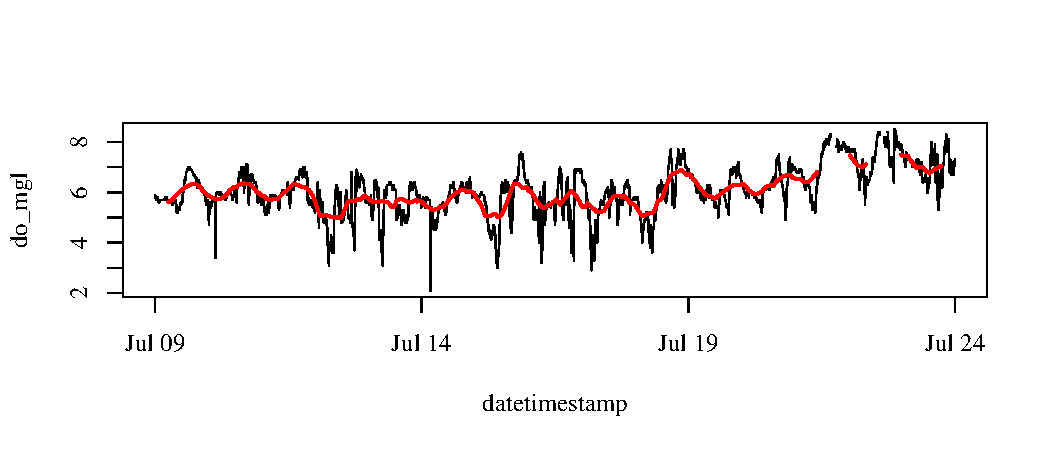
\includegraphics[width=\maxwidth]{figure/smooth_ex} 

}

\caption[Raw and smoothed dissolved oxygen data for a two-week period after using the \texttt{smoother} function]{Raw and smoothed dissolved oxygen data for a two-week period after using the \texttt{smoother} function.\label{fig:smooth_ex}}
\end{figure}


\end{knitrout}

A common issue with any statistical analysis is the treatment of missing values.  Missing data can be excluded from the analysis, included but treated as true zeroes, or interpolated based on similar values.  In either case, an analyst should have a strong rationale for the chosen method.  A common approach implemented in the SWMPr package is linear interpolation using the \texttt{na.approx} function (\Cref{fig:interp_ex}).  A simple curve fitting method is used to create a continuous set of records between observations separated by missing data.  However, the ability of the interpolated data to approximate actual trends is related to the maximum gap size between observations with missing data.  Interpolation between larger gaps are less likely to resemble patterns of an actual parameter, whereas interpolation between smaller gaps are often more accurate.  An upper limit on the maximum gap size to interpolate trends depends on the characteristics of the dataset such that a trial and error approach is appropriate for most applications.  The \texttt{maxgap} argument passed to \texttt{na.approx} defines the maximum gap size for interpolation and the following illustrates use of different maximum values to fill missing data.  

\begin{knitrout}\small
\definecolor{shadecolor}{rgb}{1, 1, 1}\color{fgcolor}\begin{kframe}
\begin{verbatim}
> # get data, qaqc and subset
> data(apadbwq)
> dat <- qaqc(apadbwq)
> dat <- subset(dat, select = 'do_mgl', 
+   subset = c('2013-01-22 00:00', '2013-01-26 00:00'))
> 
> # interpolate, maxgap of 10 records
> fill1 <- na.approx(dat, params = 'do_mgl', maxgap = 10)
> 
> # interpolate maxgap of 30 records
> fill2 <- na.approx(dat, params = 'do_mgl', maxgap = 30)
> 
> # plot for comparison
> par(mfrow = c(3, 1))
> plot(dat, main = 'Raw')
> plot(fill1, col = 'red', main = 'Interpolation - maximum gap of 10 records')
> lines(dat)
> plot(fill2, col = 'red', main = 'Interpolation - maximum gap of 30 records')
> lines(dat)
\end{verbatim}
\end{kframe}\begin{figure}[!ht]


{\centering 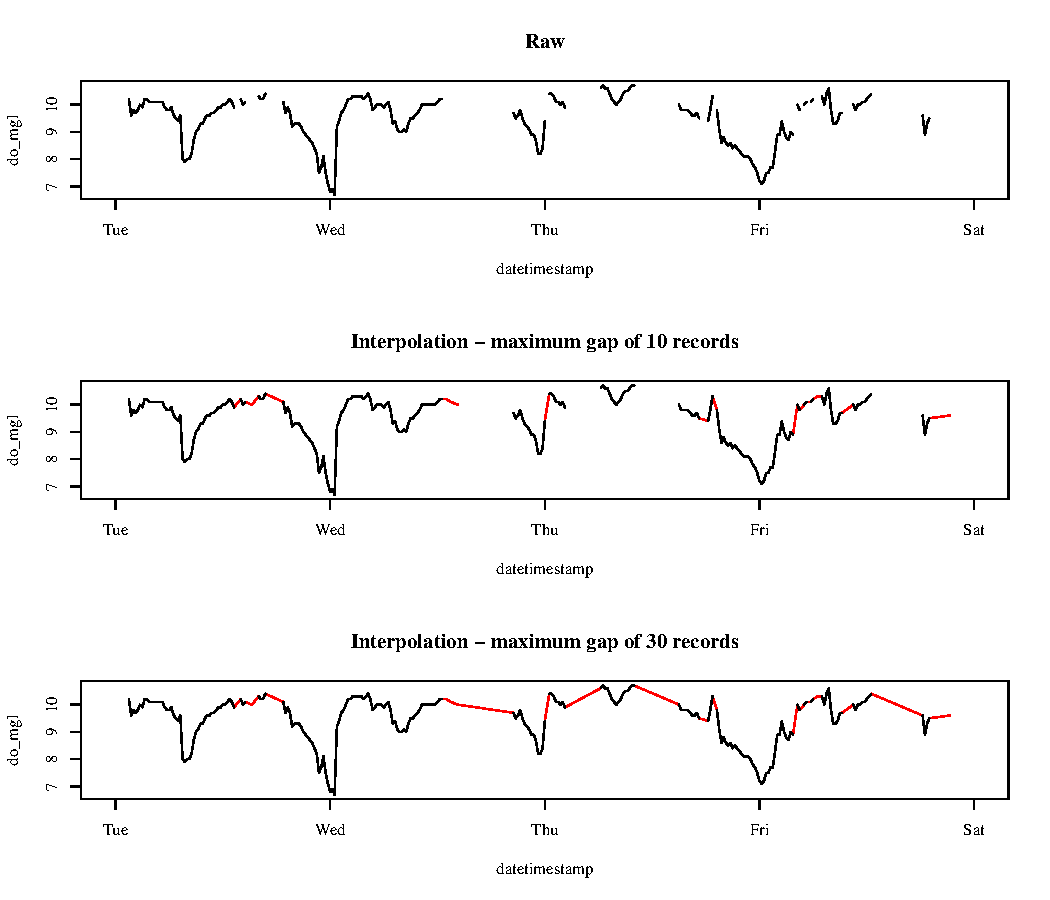
\includegraphics[width=\maxwidth]{figure/interp_ex} 

}

\caption[Examples illustrating use of the \texttt{na.approx} function to fill gaps of different sizes in a dissolved oxygen time series for a four day period.]{Examples illustrating use of the \texttt{na.approx} function to fill gaps of different sizes in a dissolved oxygen time series for a four day period.\label{fig:interp_ex}}
\end{figure}


\end{knitrout}

The disaggregation of time series into additive or multiplicative components that can be attributed to separate sources of variance is another common application for trend analysis.  The \texttt{decomp} function is a simple wrapper to \texttt{decompose} \cite{Kendall83} that separates a time series into components describing a trend, cyclical variation (e.g., daily or annual), and the remainder  (\Cref{fig:decomp_ex1}).  An additive decomposition assumes that the cyclical component of the time series is stationary (i.e., the variance is constant), otherwise a multiplicative decomposition can be used.  The \texttt{frequency} argument describes the periodicity of the cyclical parameter in units of the native time step.  For example, the \texttt{frequency} for a parameter with daily periodicity would be 96 if the time step is 15 minutes (24 hours * 60 minutes / 15 minutes).  The frequency of a parameter with annual periodicity at a 15 minute time step would be 35040 (365 days * 24 hours * 60 minutes / 15 minutes).  For simplicity, character strings of \texttt{`daily'} or \texttt{`annual'} can be supplied in place of numeric values, although any number can be used to identify an arbitrary cyclical component.  A starting value of the time series must be supplied in the latter case that indicates the sequence in the cycle for the first observation (e.g., 1 if the the first observation is at sunrise for a diurnal cycle).\footnote{The value is passed to the \texttt{ts} function, \url{https://stat.ethz.ch/R-manual/R-devel/library/stats/html/ts.html}}  Use of the \texttt{setstep} function is also required to standardize the time step prior to decomposition.

\begin{knitrout}\small
\definecolor{shadecolor}{rgb}{1, 1, 1}\color{fgcolor}\begin{kframe}
\begin{verbatim}
> # get data
> data(apadbwq)
> swmp1 <- apadbwq
> 
> # subset for daily decomposition
> dat <- subset(swmp1, subset = c('2013-07-01 00:00', '2013-07-31 00:00'))
> 
> # decomposition and plot
> test <- decomp(dat, param = 'do_mgl', frequency = 'daily')
> plot(test)
\end{verbatim}
\end{kframe}\begin{figure}[!ht]


{\centering 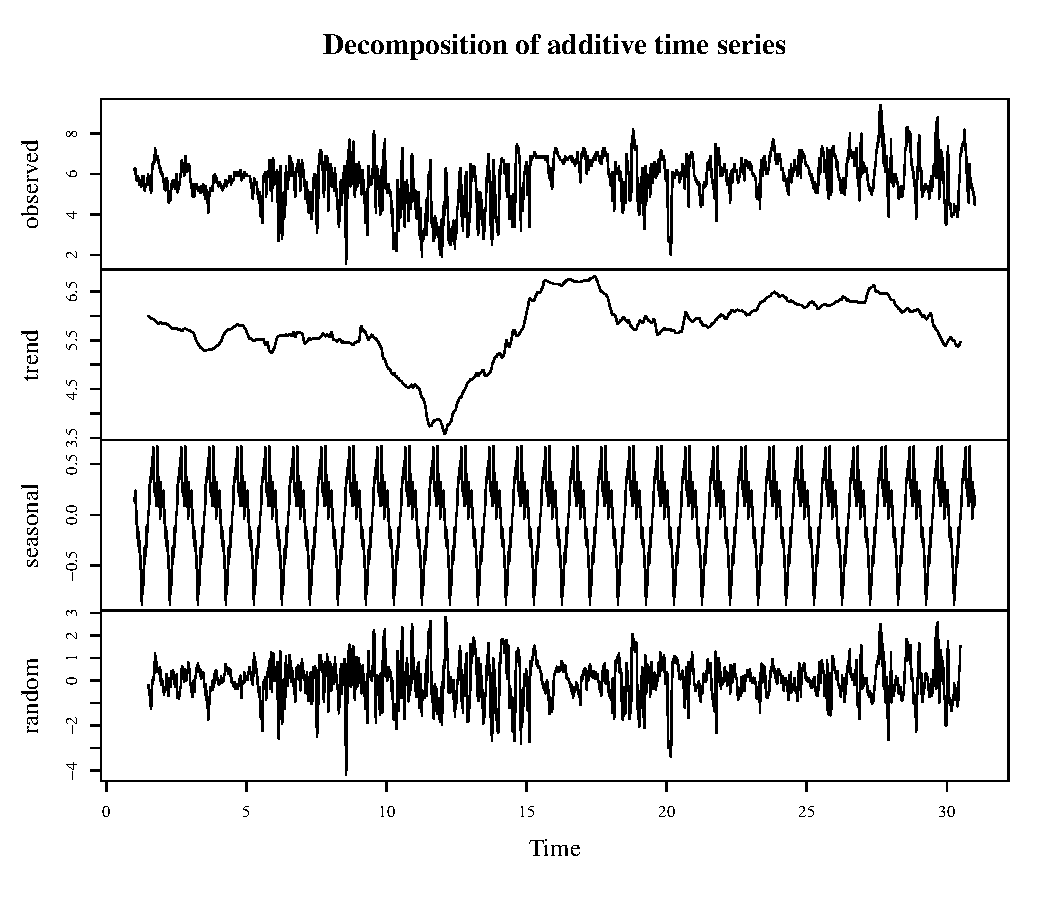
\includegraphics[width=\maxwidth]{figure/decomp_ex1} 

}

\caption[An additive decomposition of dissolved oxygen into a trend, seasonal, and random component using the \texttt{decomp} function]{An additive decomposition of dissolved oxygen into a trend, seasonal, and random component using the \texttt{decomp} function.\label{fig:decomp_ex1}}
\end{figure}


\end{knitrout}

An alternative approach to time series decomposition is provided by the \texttt{decomp\_cj} function, which is a simple wrapper to the \texttt{decompTs} function in the wq package \cite{Cloern10,Jassby14}.  The \texttt{decomp\_cj} function provides only a monthly decomposition, which is appropriate for characterizing relatively long-term trends.  This approach works best for nutrient data that are typically obtained on a monthly cycle.  The function will also work with continuous water quality or weather data but note that the data must first be aggregated on the monthly scale before decomposition.  Additionally, the time series is decomposed into the grandmean, annual, seasonal, and events components, as compared to trend, seasonal, and random components for the \texttt{decomp} function described above.  For both, the random or events components can be considered anomalies that do not follow the trends in the remaining categories.  Additional arguments passed to \texttt{decompTs} can be used with \texttt{decomp\_cj}, such as \texttt{startyr}, \texttt{endyr}, and \texttt{type}.  Values passed to \texttt{type} are \texttt{mult} (default) or \texttt{add}, referring to multiplicative or additive decomposition.  \Cref{fig:decomp_ex2} shows the results from the \texttt{decomp\_cj} function applied to a multi-year chlorophyll time series.

\begin{knitrout}\small
\definecolor{shadecolor}{rgb}{1, 1, 1}\color{fgcolor}\begin{kframe}
\begin{verbatim}
> # get data
> data(apacpnut)
> dat <- apacpnut
> dat <- qaqc(dat, qaqc_keep = NULL)
> 
> # decomposition of chl
> decomp_cj(dat, param = 'chla_n')
\end{verbatim}
\end{kframe}\begin{figure}[!ht]


{\centering 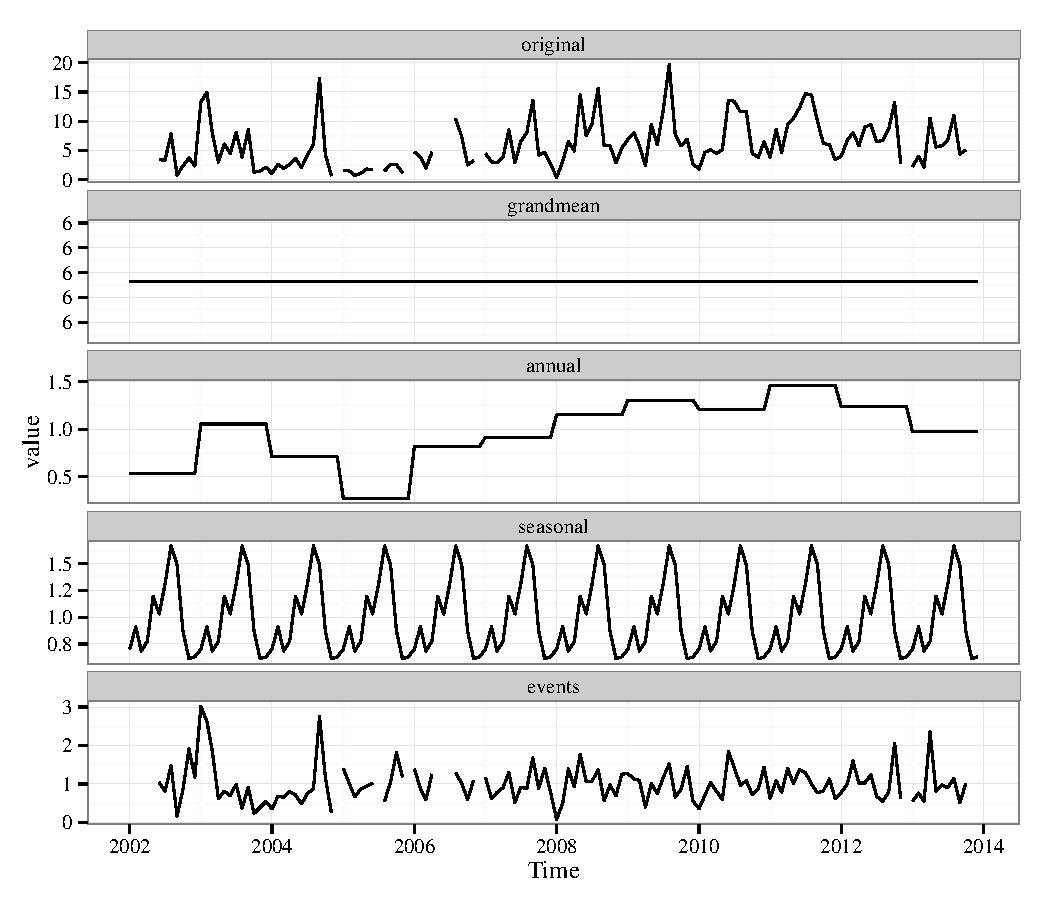
\includegraphics[width=\maxwidth]{figure/decomp_ex2} 

}

\caption[Additive decomposition of a multi-year chlorophyll time series into the grandmean, annual, seasonal, and events components using the \texttt{decomp\_cj} function]{Additive decomposition of a multi-year chlorophyll time series into the grandmean, annual, seasonal, and events components using the \texttt{decomp\_cj} function.\label{fig:decomp_ex2}}
\end{figure}


\end{knitrout}

Detailed exploratory graphics are also useful for evaluating general trends in observed data.  Several graphics showing seasonal and annual trends for a single SWMP parameter can be obtained using the \texttt{plot\_summary} function (\Cref{fig:summary_ex}).  The plots include monthly distributions, monthly anomalies, and annual anomalies in multiple formats.  Anomalies are defined as the difference between the monthly or annual averages from the grand mean for the parameter.  An interactive web application \cite{Chang15} that uses this function is available for viewing results of any parameter at all \ac{SWMP} sites (see the \nameref{supp_info}).

\begin{knitrout}\small
\definecolor{shadecolor}{rgb}{1, 1, 1}\color{fgcolor}\begin{kframe}
\begin{verbatim}
> ## import data
> data(apacpnut)
> dat <- qaqc(apacpnut)
> 
> ## plot
> plot_summary(dat, param = 'chla_n', years = c(2007, 2013))
\end{verbatim}
\end{kframe}\begin{figure}[!ht]


{\centering 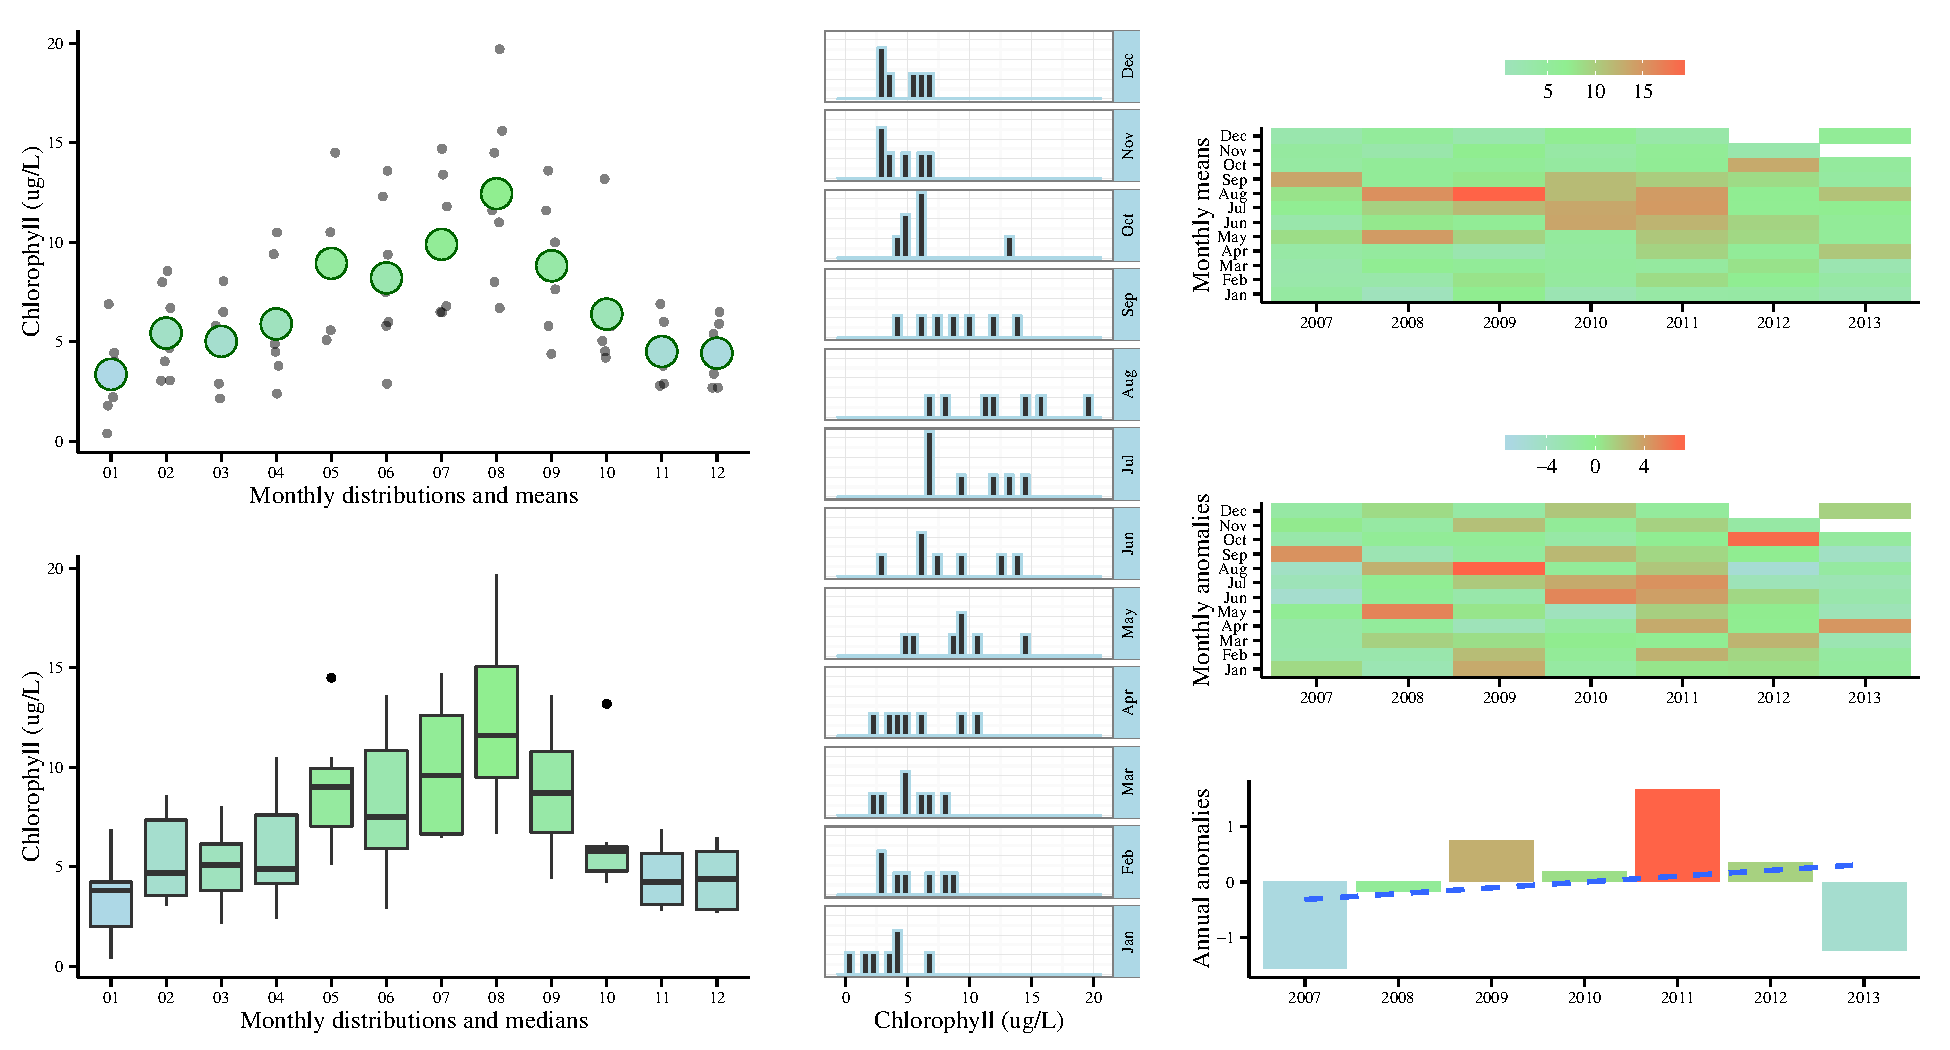
\includegraphics[width=\maxwidth]{figure/summary_ex} 

}

\caption[Summaries of a multi-year chlorophyll time series using the \texttt{plot\_summary} function]{Summaries of a multi-year chlorophyll time series using the \texttt{plot\_summary} function.  Summaries include monthly distributions (means on top left, quantiles on bottom left), monthly histograms (center), monthly means by year (top right), deviation from monthly means (middle right), and annual trends as deviations from the grand mean (bottom right)\label{fig:summary_ex}}
\end{figure}


\end{knitrout}

Finally, estimates of ecosystem metabolism provide a measure of overall system productivity to evaluate whether an ecosystem is a net source or sink of organic material.  The open-water method \cite{Odum56} is a common approach to quantify metabolism using a mass balance equation that describes the change in dissolved oxygen over time from the balance between photosynthetic and respiration processes, corrected using an empirically constrained air-sea gas diffusion model \cite{Ro06,Thebault08}. The diffusion-corrected \ac{DO} flux estimates are averaged separately over each day and night of the time series. The nighttime average \ac{DO} flux is used to estimate respiration rates, while the daytime \ac{DO} flux is used to estimate net primary production. To generate daily integrated rates, respiration rates are assumed constant such that hourly night time \ac{DO} flux rates are multiplied by 24. Similarly, the daytime \ac{DO} flux rates are multiplied by the number of daylight hours, which varies with location and time of year, to yield net daytime primary production. Respiration rates are subtracted from daily net production estimates to yield gross production rates. The metabolic day is considered the 24 hour period between sunsets on two adjacent calendar days  

The \texttt{ecometab} function is used to implement the open-water method with a combined water quality and weather dataset \cite{Caffrey14}.  Several assumptions must be met for a valid interpretation of the results.  First, the \ac{DO} time series is assumed to be a sample of the same water mass over time.  Tidal advection may have a significant influence on the time series, which can contribute to a significant amount of noise in metabolic estimates.  The extent to which tidal advection influences the dissolved oxygen signal depends on various site-level characteristics and an intimate knowledge of the site may be required.  Second, areal rates for gross production and total respiration are based on volumetric rates normalized to the depth of the water column at the sampling location, which is assumed to be well-mixed, such that the water quality sensor is reflecting the integrated processes in the entire water column (including the benthos).  Water column depth is calculated as the mean value of the depth variable across the time series in the \texttt{swmpr} object. Depth values are floored at one meter for very shallow stations and 0.5 meters is also added to reflect the practice of placing sensors slightly off of the bottom.  Third, the air-sea gas exchange model is calibrated with wind data either collected at, or adjusted to, wind speed at 10 m above the surface.  The metadata should be consulted for exact height. Other assumptions may apply and relevant resources should be consulted to ensure appropriate application of the open-water method (see \cite{Kemp12,Needoba12}).

The following is an example that shows use of the function from a combined water quality and weather data set.  Monthly aggregations of the raw, daily estimates are plotted using \texttt{plot\_metab} (\Cref{fig:metab_ex}).

\begin{knitrout}\small
\definecolor{shadecolor}{rgb}{1, 1, 1}\color{fgcolor}\begin{kframe}
\begin{verbatim}
> ## import water quality and weather data
> data(apadbwq)
> data(apaebmet)
> 
> ## qaqc, combine
> wq <- qaqc(apadbwq)
> met <- qaqc(apaebmet)
> dat <- comb(wq, met)
> 
> ## estimate metabolism
> res <- ecometab(dat, trace = FALSE)
> plot_metab(res)
\end{verbatim}
\end{kframe}\begin{figure}[!ht]


{\centering 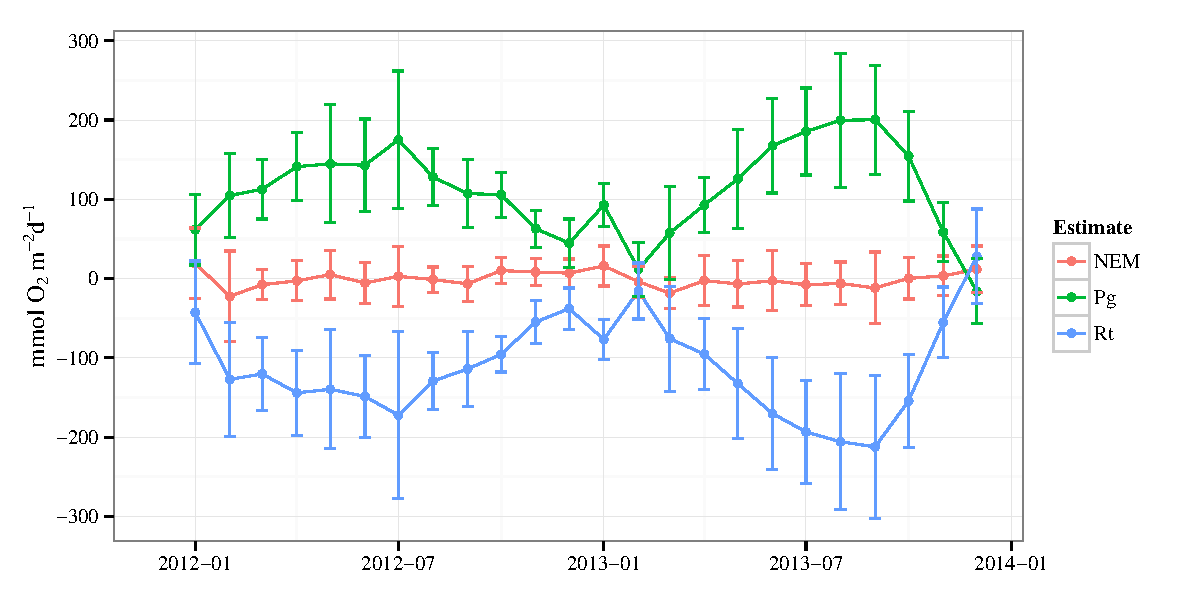
\includegraphics[width=\maxwidth]{figure/metab_ex} 

}

\caption[Monthly means (95\% confidence) of ecosystem metabolism estimates (net ecosystem metabolism, gross production, and total respiration) for combined water quality and weather data for two years at Apalachicola Bay, Florida]{Monthly means (95\% confidence) of ecosystem metabolism estimates (net ecosystem metabolism, gross production, and total respiration) for combined water quality and weather data for two years at Apalachicola Bay, Florida.\label{fig:metab_ex}}
\end{figure}


\end{knitrout}

Finally, the \texttt{map\_reserve} function can be used to create a map with all stations at a reserve using functions in the ggmap package \cite{Kahle13}. This map may be useful for aiding the interpretation of spatial trends in water quality parameters given the relative locations in a reserve.  The current function is limited to Google maps of four types that can be set with the \texttt{map\_type} argument: terrain (default), satellite, roadmap, or hybrid.  The \texttt{zoom} argument can be chosen through trial and error depending on the spatial extent of the reserve.  See the help documentation for the \texttt{ggmap} function for more info on \texttt{zoom}.

\begin{knitrout}\small
\definecolor{shadecolor}{rgb}{1, 1, 1}\color{fgcolor}\begin{kframe}
\begin{verbatim}
> # plot the stations at Jacques Cousteau reserve
> map_reserve('jac')
\end{verbatim}
\end{kframe}\begin{figure}[!ht]


{\centering 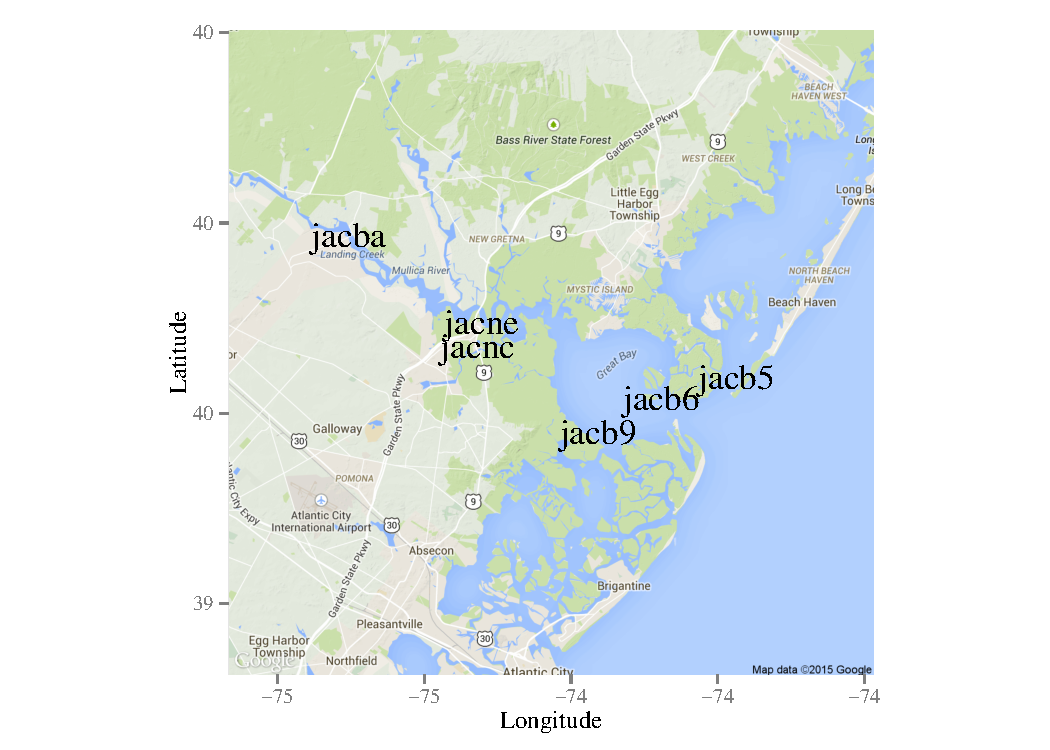
\includegraphics[width=\maxwidth]{figure/map_ex} 

}

\caption[Locations of all sites at the Jacques Cousteau reserve using the \texttt{map\_reserve} function]{Locations of all sites at the Jacques Cousteau reserve using the \texttt{map\_reserve} function.\label{fig:map_ex}}
\end{figure}


\end{knitrout}

\subsection*{Miscellaneous functions}

Several additional functions are provided that do not fit the above categories (\Cref{tab:misc}).  These functions are generally used within the main functions but may be useful for more customized evaluation of \ac{SWMP} data.  

% table for misc functions
%latex.default(to_tab[, "Description", drop = F], file = "", caption = "Miscellaneous functions available from the SWMPr package.  Most are used within the main functions above but may be useful for customized evaluations of \\ac{SWMP} data.  Full documentation for each function is in the help file (e.g., execute \\texttt{?calckl} at the command line).",     rowlabel = "Function", colheads = "Description", rowname = to_tab$Functions,     caption.loc = "top", col.just = c("p{3.5in}"), label = "tab:misc",     table.env = FALSE)%
\begin{table}[!tbp]
\caption{Miscellaneous functions available from the SWMPr package.  Most are used within the main functions above but may be useful for customized evaluations of \ac{SWMP} data.  Full documentation for each function is in the help file (e.g., execute \texttt{?calckl} at the command line).\label{tab:misc}} 
\begin{center}
\begin{tabular}{lp{3.5in}}
\hline\hline
\multicolumn{1}{l}{Function}&\multicolumn{1}{c}{Description}\tabularnewline
\hline
\texttt{calckl}&Estimate the reaeration coefficient for air-sea gas exchange.  Used in the \texttt{ecometab} function.\tabularnewline
\texttt{metab\_day}&Identify the metabolic day for each approximate 24 period in an hourly time series.  Used in the \texttt{ecometab} function.\tabularnewline
\texttt{param\_names}&Returns column names as a list for the parameter types (nutrients, weather, or water quality).  Includes \ac{QAQC} columns with \texttt{f\_} prefix. Used in the data retrieval functions.\tabularnewline
\texttt{parser}&Parses HTML returned from \ac{CDMO} data requests.  Used in the retrieval functions.\tabularnewline
\texttt{swmpr}&Creates a \texttt{swmpr} object class.  Used in the data retrieval functions.\tabularnewline
\texttt{time\_vec}&Converts time vectors to \texttt{POSIXct} objects with the appropriate time zone for a site.  Used in the data retrieval functions.\tabularnewline
\hline
\end{tabular}\end{center}

\end{table}


\section*{Applications using the SWMPr package}
\label{swmp_apps}

This section describes three examples using the SWMPr package to illustrate the improved ability to synthesize and evaluate multi-year time series of estuarine data. First, the open-water method for estimating metabolism was applied to nearly all co-located water quality and weather sites at each \ac{NERRS} reserve using all years of available data.  The results are provided primarily to illustrate ease of use of the functions and secondarily to provide an update on metabolism estimates using the most recent \ac{SWMP} data.  Caffrey \cite{Caffrey03} and Caffrey \cite{Caffrey04} applied the open-water method to estimate ecosystem metabolism using five years of water quality observations at two sites at each of the \ac{NERRS} reserves.  The air-sea gas exchange model also assumed a constant value for the reaeration coefficient, whereas the current \texttt{ecometab} function provides a more accurate estimate by including weather data in the calculation (see Caffrey et al. \cite{Caffrey14} for details).

Water quality and weather observations from January 1995 to December 2014 for all \ac{NERRS} sites were obtained through a bulk data request using the zip downloads feature of \ac{CDMO}.  All csv files for each station were imported into R using the \texttt{import\_local} function, processed using the \texttt{setstep} and \texttt{qaqc} functions, then saved locally as binary RData files.\footnote{Data processing script: \url{https://github.com/fawda123/swmp_rats/blob/master/R/dat_proc.R}} This resulted in a single \texttt{swmpr} object for each parameter at each site.  All files were then uploaded to a remote server for online access.  An additional R script\footnote{Metabolism processing script: \url{https://gist.github.com/fawda123/4fc51c2cb86341ed9291}} was executed that retrieved and processed water quality and weather data at each reserve to estimate metabolism.  Two water quality sites with the longest time series at each reserve were used.  Mean annual values at each site, organized by region, are shown in \Cref{fig:metab_plo}, whereas decadal comparisons are shown in \Cref{tab:metab_tab}.  All sites were generally net heterotrophic across the range of observations (i.e., sink of organic matter, in agreement with Caffrey \cite{Caffrey03}), although differences were observed in early (i.e., 1995-2004) as compared to recent (2005-2014) time periods. Overall, the results indicate that between-region and within-site differences in metabolism are apparent and varying by time period, such that a more comprehensive evaluation of factors that influence metabolic rates is needed.  More importantly, use of the data retrieval, synthesis, and analysis functions to create the results illustrates the utility provided by the SWMPr package.

% metabolism figure
\begin{knitrout}\small
\definecolor{shadecolor}{rgb}{1, 1, 1}\color{fgcolor}\begin{figure}[!ht]


{\centering 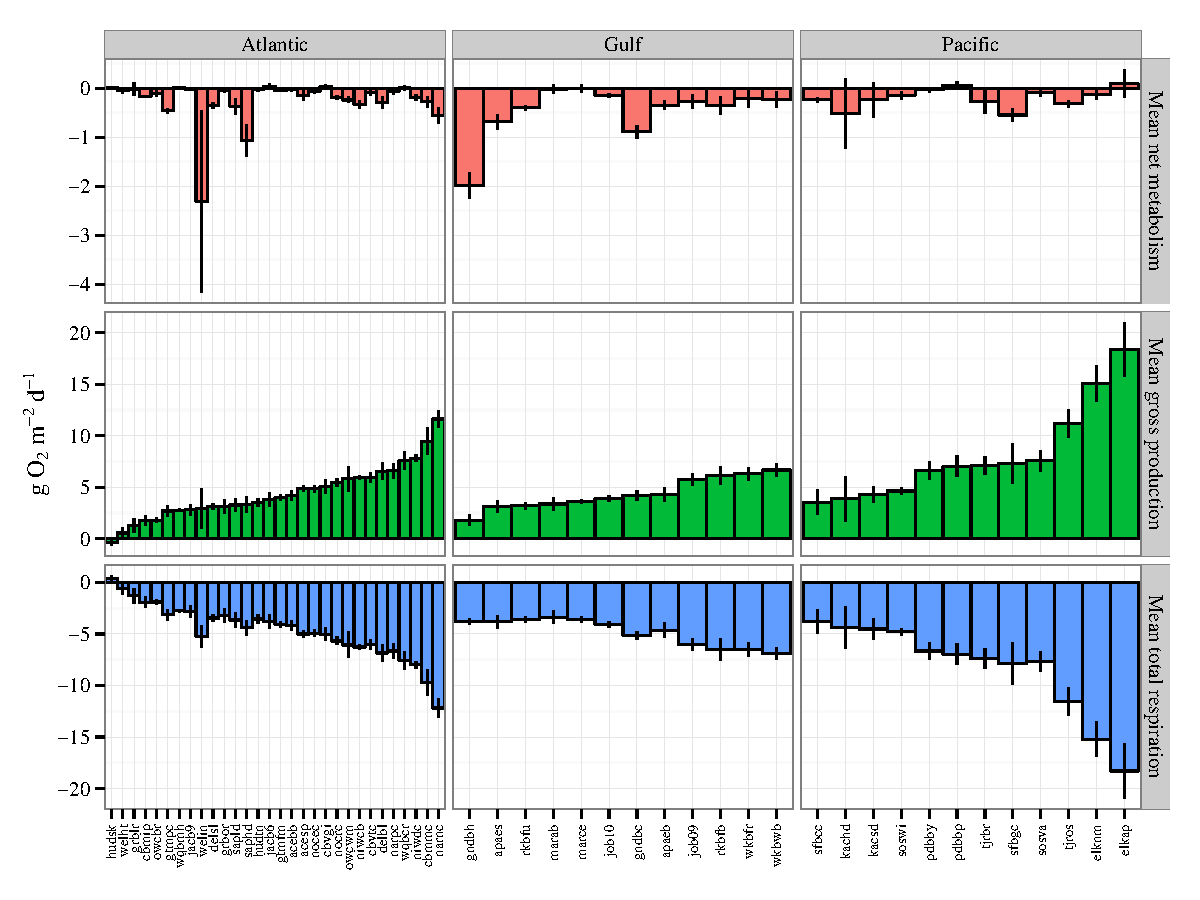
\includegraphics[width=\textwidth]{figure/metab_plo} 

}

\caption[Aggregated estimates of net metabolism, gross production, and total respiration for two sites at each \ac{NERRS} reserve]{Aggregated estimates of net metabolism, gross production, and total respiration for two sites at each \ac{NERRS} reserve.  Values are daily integrated estimates as mean annual values averaged across all years with 95\% confidence intervals.  Two sites were chosen from each reserve that had the longest available time series. Sites were assigned to regions based on approximate geographic coordinates.\label{fig:metab_plo}}
\end{figure}


\end{knitrout}

% table summary of trends
%latex.default(metabs_tab[, !names(metabs_tab) %in% c("site",     "region")], file = "", caption = cap, cgroup = c("NEM\\textsuperscript{{\\it a}}",     "Pg", "Rt"), n.cgroup = c(2, 2, 2), colheads = rep(c("1995-2004",     "2005-2014"), 3), rowlabel = "Site", rowname = metabs_tab$site,     digits = 2, insert.bottom = foots, rgroup = unique(metabs_tab$region),     n.rgroup = nrgroups, label = "tab:metab_tab", size = "footnotesize")%
\begin{table}[!tbp]
{\footnotesize
\caption{Trends in metabolism for two sites at each of the \ac{NERRS} reserves.  Values are averages of mean annual estimates for each period of observation (1994-2004 and 2005-2014). Bold values indicate an increase from the first period, whereas italic values indicate a decrease. Sites were assigned to regions based on approximate geographic coordinates.\label{tab:metab_tab}} 
\begin{center}
\begin{tabular}{lllcllcll}
\hline\hline
\multicolumn{1}{l}{\bfseries Site}&\multicolumn{2}{c}{\bfseries NEM\textsuperscript{{\it a}}}&\multicolumn{1}{c}{\bfseries }&\multicolumn{2}{c}{\bfseries Pg}&\multicolumn{1}{c}{\bfseries }&\multicolumn{2}{c}{\bfseries Rt}\tabularnewline
\cline{2-3} \cline{5-6} \cline{8-9}
\multicolumn{1}{l}{}&\multicolumn{1}{c}{1995-2004}&\multicolumn{1}{c}{2005-2014}&\multicolumn{1}{c}{}&\multicolumn{1}{c}{1995-2004}&\multicolumn{1}{c}{2005-2014}&\multicolumn{1}{c}{}&\multicolumn{1}{c}{1995-2004}&\multicolumn{1}{c}{2005-2014}\tabularnewline
\hline
{\bfseries Atlantic}&&&&&&&&\tabularnewline
~~acebb&-0.04&{\bf -0.03}&&5.11&{\it 3.81}&&-5.15&{\bf -3.82}\tabularnewline
~~acesp&-0.26&{\bf -0.1}&&4.68&{\bf 4.93}&&-4.94&{\it -5.03}\tabularnewline
~~cbmip&-0.14&{\it -0.17}&&1.02&{\bf 1.91}&&-1.16&{\it -2.08}\tabularnewline
~~cbmmc&-0.43&{\bf -0.24}&&6.06&{\bf 10.13}&&-6.48&{\it -10.38}\tabularnewline
~~cbvgi&0.13&{\it 0}&&6.56&{\it 4.47}&&-6.43&{\bf -4.46}\tabularnewline
~~cbvtc&-0.15&{\bf -0.07}&&5.58&{\bf 6.07}&&-5.73&{\it -6.14}\tabularnewline
~~delbl&-0.59&{\bf -0.16}&&6.68&{\it 6.51}&&-7.27&{\bf -6.67}\tabularnewline
~~delsl&-0.37&{\bf -0.33}&&2.84&{\bf 3.22}&&-3.21&{\it -3.55}\tabularnewline
~~grblr&&-0.02&&&1.28&&&-1.31\tabularnewline
~~grbor&&-0.04&&&3.16&&&-3.2\tabularnewline
~~gtmfm&-0.09&{\bf -0.04}&&3.36&{\bf 4.19}&&-3.45&{\it -4.23}\tabularnewline
~~gtmpc&-0.48&{\bf -0.45}&&1.95&{\bf 2.91}&&-2.43&{\it -3.37}\tabularnewline
~~hudsk&0.02&{\it 0.02}&&-0.36&{\it -0.39}&&0.38&{\bf 0.41}\tabularnewline
~~hudtn&-0.03&{\it -0.03}&&3.75&{\it 3.43}&&-3.78&{\bf -3.46}\tabularnewline
~~jacb6&0.05&{\it 0.03}&&3.41&{\bf 3.93}&&-3.36&{\it -3.89}\tabularnewline
~~jacb9&0.01&{\it -0.02}&&1.8&{\bf 3.1}&&-1.79&{\it -3.12}\tabularnewline
~~narnc&-0.64&{\bf -0.53}&&12.64&{\it 11.33}&&-13.25&{\bf -11.86}\tabularnewline
~~narpc&-0.14&{\bf -0.03}&&7.36&{\it 6.3}&&-7.5&{\bf -6.32}\tabularnewline
~~niwcb&-0.46&{\bf -0.28}&&5.5&{\bf 6.1}&&-5.95&{\it -6.38}\tabularnewline
~~niwdc&-0.13&{\it -0.2}&&7.28&{\bf 8.02}&&-7.41&{\it -8.23}\tabularnewline
~~nocec&-0.05&{\it -0.06}&&4.86&{\bf 4.88}&&-4.92&{\it -4.94}\tabularnewline
~~nocrc&-0.19&{\it -0.19}&&5.93&{\it 5.31}&&-6.12&{\bf -5.5}\tabularnewline
~~owcbr&-0.17&{\bf -0.09}&&1.45&{\bf 1.9}&&-1.62&{\it -1.99}\tabularnewline
~~owcwm&-0.36&{\bf -0.19}&&7.02&{\it 5.36}&&-7.38&{\bf -5.54}\tabularnewline
~~saphd&-1.28&{\bf -1}&&1.89&{\bf 3.77}&&-3.17&{\it -4.77}\tabularnewline
~~sapld&-0.16&{\it -0.43}&&2.32&{\bf 3.56}&&-2.49&{\it -3.99}\tabularnewline
~~welht&-0.07&{\bf -0.04}&&0.36&{\bf 0.63}&&-0.43&{\it -0.67}\tabularnewline
~~welin&-1.87&{\it -2.49}&&3.61&{\it 2.68}&&-5.48&{\bf -5.18}\tabularnewline
~~wqbcr&-0.01&{\bf 0.01}&&8.13&{\it 7.41}&&-8.14&{\bf -7.4}\tabularnewline
~~wqbmh&0.02&{\it 0}&&2.82&{\it 2.76}&&-2.79&{\bf -2.75}\tabularnewline
\hline
{\bfseries Gulf}&&&&&&&&\tabularnewline
~~apaeb&-0.35&{\it -0.35}&&4.19&{\bf 4.31}&&-4.54&{\it -4.67}\tabularnewline
~~apaes&-0.71&{\bf -0.67}&&3.35&{\it 3.05}&&-4.06&{\bf -3.73}\tabularnewline
~~gndbc&-1.02&{\bf -0.88}&&3.5&{\bf 4.3}&&-4.51&{\it -5.18}\tabularnewline
~~gndbh&-1.81&{\it -2}&&2.19&{\it 1.77}&&-4&{\bf -3.77}\tabularnewline
~~job09&-0.34&{\bf -0.25}&&5.32&{\bf 5.95}&&-5.66&{\it -6.2}\tabularnewline
~~job10&-0.15&{\it -0.15}&&3.58&{\bf 4.03}&&-3.72&{\it -4.2}\tabularnewline
~~marab&&-0.02&&&3.38&&&-3.4\tabularnewline
~~marce&&-0.01&&&3.62&&&-3.63\tabularnewline
~~rkbfb&-0.28&{\it -0.37}&&5.28&{\bf 6.25}&&-5.56&{\it -6.62}\tabularnewline
~~rkbfu&-0.33&{\it -0.41}&&2.95&{\bf 3.24}&&-3.28&{\it -3.64}\tabularnewline
~~wkbfr&-0.29&{\bf -0.14}&&6.27&{\bf 6.35}&&-6.57&{\bf -6.49}\tabularnewline
~~wkbwb&-0.29&{\bf -0.16}&&6.81&{\it 6.54}&&-7.1&{\bf -6.69}\tabularnewline
\hline
{\bfseries Pacific}&&&&&&&&\tabularnewline
~~elkap&0.03&{\bf 0.11}&&14.7&{\bf 19.84}&&-14.67&{\it -19.74}\tabularnewline
~~elknm&-0.24&{\bf -0.08}&&11.95&{\bf 16.37}&&-12.18&{\it -16.45}\tabularnewline
~~kachd&0.2&{\it -0.66}&&7.31&{\it 3.2}&&-7.12&{\bf -3.86}\tabularnewline
~~kacsd&-0.06&{\it -0.26}&&5.15&{\it 4.2}&&-5.21&{\bf -4.45}\tabularnewline
~~pdbbp&0.01&{\bf 0.08}&&6.29&{\bf 7.31}&&-6.27&{\it -7.23}\tabularnewline
~~pdbby&-0.07&{\bf -0.01}&&8.39&{\it 5.92}&&-8.47&{\bf -5.93}\tabularnewline
~~sfbcc&&-0.24&&&3.56&&&-3.79\tabularnewline
~~sfbgc&&-0.55&&&7.32&&&-7.87\tabularnewline
~~sosva&-0.2&{\bf -0.05}&&6.98&{\bf 7.83}&&-7.18&{\it -7.87}\tabularnewline
~~soswi&-0.28&{\bf -0.08}&&4.41&{\bf 4.74}&&-4.69&{\it -4.82}\tabularnewline
~~tjrbr&-1.33&{\bf -0.17}&&7.72&{\it 7.06}&&-9.05&{\bf -7.22}\tabularnewline
~~tjros&-0.26&{\it -0.34}&&10.18&{\bf 11.61}&&-10.44&{\it -11.96}\tabularnewline
\hline
\end{tabular}\end{center}}

\footnotesize{\textsuperscript{{\it a}}NEM: net ecosystem metabolism, Pg: gross production, Rt: total respiration, all values in g O$_2$ m$^{-2}$ d$^{-1}$ as annual averages.}\end{table}


The second and third examples are two interactive web applications \cite{Chang15} created using the SWMPr package that illustrate summaries and comparisons of \ac{SWMP} data (see the \nameref{supp_info}).  The first web application evaluates trends in \ac{SWMP} data within and between sites using an interactive map.  Trends between reserves can be viewed using the map, whereas trends at individual sites can be viewed by clicking on a map location.  Site-level trends are shown below the map with a simple linear regression to show an increase or decrease in values over time.  Trends on the map at each station are plotted as circles that identify the direction and significance of the trend, such that larger points with darker colors indicate a strong trend.  The trend direction is blue for decreasing and red for increasing with time.  The second application provides graphical summaries of water quality, weather, or nutrient station data at individual stations using the \texttt{plot\_summary} function. The drop down menus can be used to select the station, date range, and parameter for plotting. The data used for each application are similar to those used to estimate ecosystem metabolism described above and are available in the \nameref{supp_info}.  

\section*{Summary}

The ability of management and research programs to address critical environmental issues is highly dependent on the quality of data used to inform decision making.  Standardized monitoring programs have vastly improved the ability to evaluate factors that influence a range of conditions, leading to more comprehensive assessments of site-specific characteristics and more informed decisions to manage environmental resources.  The \acl{SWMP} has provided twenty years of continuous monitoring of environmental characteristics at over over 140 stations within the 28 estuaries of the \acl{NERRS}.  This monitoring network establishes a foundation  for more effective coastal management by providing standardized data to address spatiotemporal variation in natural and anthropogenic characteristics that influence environmental condition.  Although the data provided by \ac{SWMP} are unique among coastal observing systems and have been used in a variety of applications \cite{Bulthius95,Caffrey03,Sanger02,Wenner04,Dix08}, the capacity of \ac{NERRS} researchers and staff to more effectively evaluate \ac{SWMP} data could be greatly improved using the SWMPr package.

The SWMPr package provides several functions to retrieve, organize, and analyze \ac{SWMP} data to more effectively address common challenges working with large datasets.  The package is designed to augment, rather than replace, existing data retrieval programs by providing a bridge betwen the raw data and the analysis software through its numerous data retrieval functions (\Cref{tab:retrieve}).  Established \ac{QAQC} methods and data processing techniques are also enhanced with SWMPr by functions that filter observations for different \ac{QAQC} flags (\texttt{qaqc}) and subset by selected dates or variables (\texttt{subset}).  Additionally, cumbersome challenges comparing differents datasets are addressed by the \texttt{setstep} and \texttt{comb} functions that standardize time steps and combine the data.  Finally, the analysis functions provide numerous tools to implement common analyses for time series and more specific methods for water quality data.  In particular, the \texttt{ecometab} function can be used to estimate daily integrated rates of ecosystem metabolism using the open-water method \cite{Odum56,Caffrey14}.  The above analysis (see \nameref{swmp_apps}) provided a cursory update of metabolism estimates for each the \ac{NERRS} estuaries using recent data to evaluate trends over time.  Although further evaluation of the data are needed, particularly regarding assumptions of the open-water method and tidal effects, the results could be used in a more comprehensive evaluation of factors that influence estuary metabolism. Further development of the SWMPr package will consider modifying existing and including additional functions to more effectively integrate data analysis with the quality of information provided by \ac{SWMP} and \ac{NERRS}. 

\section*{Supporting Information}
\label{supp_info}

\subsection*{Trends in \ac{SWMP} parameters}
\label{swmp_trends}
Evaluate trends within and between reserves using an interactive map: \href{https://beckmw.shinyapps.io/swmp_comp}{https://beckmw.shinyapps.io/swmp\_comp}

\subsection*{Monthly and annual summary of \ac{SWMP} parameters}
\label{swmp_summary}
Summarize trends in \ac{SWMP} parameters for an individual site: \href{https://beckmw.shinyapps.io/swmp_summary/}{https://beckmw.shinyapps.io/swmp\_summary/} 

\subsection*{\ac{SWMP} data as R binary files}

Quickly access all \ac{SWMP} data from 1995 through 2014. See the help file for \texttt{import\_remote} for more information: \href{https://s3.amazonaws.com/swmpalldata/}{https://s3.amazonaws.com/swmpalldata/}

\subsection*{Source code for reproducing figures/tables}

Source code as an R script for reproducing figures and tables in the manuscript: \href{}{}

\section*{Acknowledgments}

I acknowledge the significant work of \ac{NERRS} researchers and staff that has allowed access to high-quality monitoring data.  Thanks to Dwayne Porter and Melissa Ide from \ac{CDMO} for maintaining the online database.  Thanks to Marie Bundy and Nikki Dix for giving me the opportunity to share this package with the broader \ac{NERRS} community.  Thanks to Todd O'Brien for the inspiration for the online widgets. Thanks to Mike Murrell and Jim Hagy III for assistance with documentation and implementation of the ecosystem metabolism functions. The views expressed in this article are those of the authors and do not necessarily reflect the views or policies of the U.S. Environmental Protection Agency.  The use of trade names or products does not constitute endorsement by the US Government.   

\nolinenumbers

\bibliography{swmpr_refs}

\end{document}
